\section{Uppgift 4}\label{sec:uppg04}

\subsection{Instruktioner}
\begin{verbatim}
4. Skriv en klass Personbil som representerar en personbil. Klassen ska
   innehålla följande 4 instansvariabler. Välj själv passande datatyp:

   bilmodell, årsmodell, registreringsnr och bilfärg

   Det ska finnas metoder för var och en av följande operationer:
   - returnera bilens modell
   - returnera bilens årsmodell
   - returnera bilens regnr
   - ändra bilens färg
   - returnera bilens färg
   - skriva ut bilens samtliga data (metodens returtyp ska vara void)

   Skriv sedan ett testprogram där du skapar 2 st personbils-objekt och sedan
   testar samtliga metoder. Objektens instansvariabler ska via konstruktorn
   initieras med följande värden:

   Bil1 : bilmodell Saab, årsmodell -90, regnr CCC222 och färg röd.
   Bil2 : bilmodell Volvo, årsmodell -99, regnr ABC988 och färg svart.
\end{verbatim}


\subsection{Kommentar}
Programmet \texttt{PersonbilGUI} skapades med verktyget \texttt{WindowBuilder}
i Eclipse Mars. Programmet visar hur typen \texttt{Color} kan användas i ett
GUI.  Metoden \texttt{toString()} används för att skriva ut färgen. Den visas
då i RGB-format. För att programmet ska skriva ut färgen som ett enkelt ord kan
en möjlig lösning nyttja en \texttt{enum} som "mappade" objekt av typen
\texttt{Color} med textsträngar av typen String. Typen kunde representera en
färg som sedan kan returneras i "fler former", t.ex. \texttt{Color} och
textsträng. 
Referenser för \texttt{Color} och \texttt{Swing}:

\mbox{Color -- The Java Language Specification, Java SE 7 Edition}
\footnote{\url{http://docs.oracle.com/javase/7/docs/api/java/awt/Color.html}}

\mbox{Swing Tutorial -- The Java Tutorials}
\footnote{\url{http://docs.oracle.com/javase/tutorial/uiswing/}}


\subsection{Källkod}
\javacode{src/Lab3Uppg04/Lab3Uppg04.java}
\caption{Lab3Uppg04.java}
\label{src:uppg04}

\javacode{src/Lab3Uppg04/Personbil.java}
\caption{Personbil.java}
\label{src:personbil}

\javacode{src/Lab3Uppg04/PersonbilGUI.java}
\caption{PersonbilGUI.java}
\label{src:personbilgui}


\subsection{Skärmdump}
\begin{figure}[htbp]
    \centering
        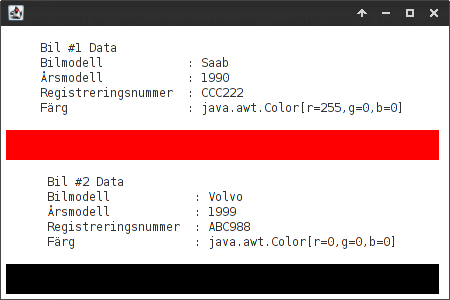
\includegraphics[width=\linewidth]{img/personbil-gui_1.png}
    \caption{Körning av \texttt{PersonbilGUI} från Uppgift~\ref{sec:uppg04}}
    \label{fig:uppg04-screenshot}
\end{figure}

\begin{figure}[htbp]
    \centering
        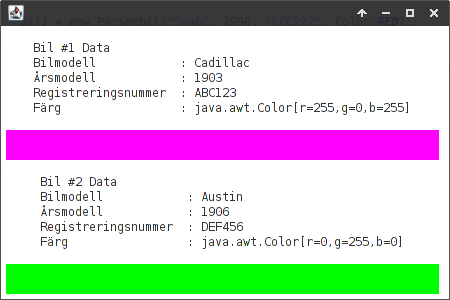
\includegraphics[width=\linewidth]{img/personbil-gui_2.png}
    \caption{Körning av \texttt{PersonbilGUI} med andra bilar}}
    \label{fig:uppg04-screenshot}
\end{figure}

